\documentclass[letterpaper,final,12pt,reqno]{amsart}

\usepackage[total={6.3in,9.2in},top=1.1in,left=1.1in]{geometry}

\usepackage{verbatim}
\usepackage{empheq}
\usepackage[dvipsnames]{xcolor}
\usepackage{animate}
\usepackage{graphicx}
\usepackage{fancyvrb}

%\usepackage{palatino}

% hyperref should be the last package we load
\usepackage[pdftex,
colorlinks=true,
plainpages=false, % only if colorlinks=true
linkcolor=blue,   % only if colorlinks=true
citecolor=Red,   % only if colorlinks=true
urlcolor=black     % only if colorlinks=true
]{hyperref}

\renewcommand{\baselinestretch}{1.05}

\newcommand{\ddt}[1]{\ensuremath{\frac{\partial #1}{\partial t}}}
\newcommand{\ddx}[1]{\ensuremath{\frac{\partial #1}{\partial x}}}
\newcommand{\ddy}[1]{\ensuremath{\frac{\partial #1}{\partial y}}}
\newcommand{\pp}[2]{\ensuremath{\frac{\partial #1}{\partial #2}}}
\renewcommand{\t}[1]{\texttt{#1}}
\newcommand{\Matlab}{\textsc{Matlab}\xspace}
\newcommand{\eps}{\epsilon}
\newcommand{\grad}{\nabla}
\newcommand{\Div}{\nabla\cdot}
\newcommand{\devstress}{\tau}
\newcommand{\RR}{\mathbb{R}}

\newcommand{\hbn}{\hat{\mathbf{n}}}

\newcommand{\bg}{\mathbf{g}}
\newcommand{\bu}{\mathbf{u}}
\newcommand{\bv}{\mathbf{v}}

\newcommand{\bX}{\mathbf{X}}



\begin{document}
\graphicspath{{../figures/}}

\title{Appendix A: A finite element Stokes solver \\ for glacier flow}

\author{Ed Bueler}

\date{\today}

\maketitle

\renewcommand{\theequation}{A\arabic{equation}}


This document is an appendix to my notes \emph{Numerical modelling of glaciers, ice sheets, and ice shelves}---here called ``the notes''---which are used for the International Summer School in Glaciology in McCarthy, Alaska.

We start by restating the Stokes model for any Glen exponent $n$, with glacier-suitable boundary conditions, and then we derive the ``weak form,'' as explained below.  A finite element (FE) method \cite{Elmanetal2014} is always based on the weak form of a differential equation.  Then we give an overview of how an FE method is set up using triangular elements for an arbitrary planar region.  We briefly discuss issues of stable mixed FE choices for Stokes problem.  We rebuild slab-on-a-slope solutions both for verification and for boundary condition purposes.  Then we describe how four open-source tools/libraries are using to generate a numerical solution:
\begin{itemize}
\item Gmsh, a mesh generator \hfill \url{http://gmsh.info/}
\item Firedrake, an FE library \hfill \url{https://www.firedrakeproject.org/}
\item PETSc, a solver library \hfill \url{http://www.mcs.anl.gov/petsc/}
\item Paraview, visualization tool \hfill \url{https://www.paraview.org/}
\end{itemize}
Finally a relatively-short Python code is shown and demonstrated.

\section{Stokes equations and the weak form}

Recall the Glen-Stokes model in equations (3), (4), (5) from the notes---also in \cite{GreveBlatter2009,JouvetRappaz2011}---but now allowing any Glen exponent $n\ge 1$:
\begin{align}
\nabla \cdot \bu &= 0 &&\text{\emph{incompressibility}} \label{incompressible} \\
- \nabla \cdot \tau + \nabla p &= \rho \bg &&\text{\emph{stress balance}} \label{forcebalance} \\
D\bu &= A_n |\tau|^{n-1} \tau &&\text{\emph{Glen flow law}} \label{flowlaw}
\end{align}
The \emph{velocity} $\bu$, \emph{pressure} $p$, \emph{ice density} $\rho$, \emph{acceleration of gravity} $\bg$, \emph{deviatoric stress tensor} $\tau$ and the \emph{strain rate tensor} $D\bu$ appear in these equations.  Note that $A_n$ in \eqref{flowlaw} is the $n$-dependent ice softness.  In Table 1 in the notes we have $A = A_3 = 10^{-16} \,\text{Pa}^{-3}\,\text{a}^{-1} = 3.1689 \times 10^{-24} \,\text{Pa}^{-3}\,\text{s}^{-1}$, and generally the units of $A_n$ are $\text{Pa}^{-n}\,\text{s}^{-1}$.

Though the notation here generally follows Table 1 in the notes, some of usage is more general or flexible especially regarding how tensors and tensor norms are used.  Here are the concrete definitions for tensor $D\bu$ and tensor norms $|D\bu|$, $|\tau|$:
\begin{align*}
(D\bu)_{ij} &= \frac{1}{2} \left((u_i)_{x_j} + (u_j)_{x_i}\right) \\
|\tau|^2 &= \frac{1}{2} \tau^\top \tau = \frac{1}{2} \tau_{ij} \tau_{ij} \\
|D\bu|^2 &= \frac{1}{2} (D\bu)^\top D\bu = \frac{1}{2} (D\bu)_{ij} (D\bu)_{ij}
\end{align*}
In the last two expressions the Einstein summation is used, either over indices $i,j=1,2,3$ or $i,j=1,2$ according to the context.  Note that the tensors $D\bu$ and $\tau$ are symmetric and have trace zero.

The deviatoric stress tensor $\tau$ is the full (Cauchy) stress tensor with the pressure removed:
    $$\sigma = \tau - p\,I$$
(One may then derive $p = -\frac{1}{3} \sigma_{ii}$, from the fact that $\tau$ has trace zero, thus that the pressure is the negative of the average normal stress, but we will not need this fact.)

Recall the viscosity form of flow law, namely equation (15) in the notes:
\begin{equation}
\tau = 2\nu D\bu = B_n |D\bu|^{\frac{1}{n} - 1} D\bu  \label{viscflowlaw}
\end{equation}
where $B_n = A_n^{-1/n}$ is the ice hardness.  With this expression we rewrite equations \eqref{forcebalance}, \eqref{flowlaw} and eliminate the deviatoric stress tensor $\tau$:
\begin{equation}
- \nabla \cdot \left(B_n |D\bu|^{\frac{1}{n} - 1} D\bu\right) + \nabla p = \rho \mathbf{g} \label{stokes}
\end{equation}

The Stokes model in strong form is, from now on, equations \eqref{incompressible} and \eqref{stokes} with certain boundary conditions.  To explain these boundary conditions consider the numerical solution shown in Figure \ref{fig:stepflowlin}

\begin{figure}
\label{fig:stepflowlin}
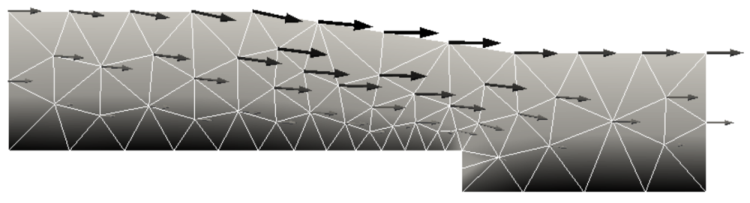
\includegraphics[width=0.95\textwidth]{stepflowlin}
\caption{A 2D Stokes problem for a glacier flowing over a bedrock step.  Arrows show velocity $\bu$ and shading is by pressure $p$.  Note the mesh of triangular finite elements.}
\end{figure}

FIXME

The model applies on a domain $\Omega\subset \RR^3$ or $\Omega \subset \RR^2$ according to the context.  This domain must have a smooth enough boundary to apply the prescribed normal stress boundary condition but it is otherwise general.  In the model the solution is the pair $(\bu,p)$ where $\bu\in V_D$ and $p \in Q$ for function spaces $V_D,Q$ precisely identified in \cite{JouvetRappaz2011}.  In fact the weak formulation of the model is proven in \cite{JouvetRappaz2011} to be well-posed under reasonable assumptions which will be satisfied in the cases we consider.

This weak formulation is derived by multiplying the equations by arbitrary test functions and then integrating by parts using the divergence theorem.  We define a nonlinear functional $F$ by multiplying \eqref{incompressible} by test function $q\in Q$ and \eqref{stokes} by test function $\bv\in V$ and combining these equations:
\begin{equation}
F(\bu,p;\bv,q) = \int_\Omega - \left(\nabla \cdot \left(B_n |D\bu|^{\frac{1}{n} - 1} D\bu\right)\right)\cdot \bv + \nabla p \cdot \bv - \rho \mathbf{g} \cdot \bv - \left(\nabla \cdot \bu\right) q \label{nonfuncone}
\end{equation}
This nonlinear functional must be zero at the solution $(\bu,p)$:
\begin{equation}
F(\bu,p;\bv,q) = 0 \qquad \text{ for all } \bv\in V \text{ and } q\in Q
\end{equation}

The integration-by-parts step uses the product rule $\nabla \cdot(f\bX) = \grad f\cdot \bX + f \nabla \cdot \bX$ and the divergence theorem $\int_\Omega \nabla \cdot \bX = \int_{\partial \Omega} \bX \cdot \hbn$.  Recalling $\tau = B_n |D\bu|^{\frac{1}{n} - 1} D\bu$ then
\begin{align*}
\int_\Omega \left(\nabla \cdot \tau\right)\cdot \bv &= \sum_{j=1}^3 \int_\Omega \nabla \cdot (\tau_{\circ j})\, v_j = \sum_{j=1}^3 \int_\Omega \nabla \cdot (\tau_{\circ j} v_j) - \tau_{\circ j} \nabla v_j \\
  &= \sum_{j=1}^3 \int_{\partial \Omega} (\tau_{\circ j} v_j) \cdot \hbn - \int_\Omega \tau_{\circ j} \nabla v_j = \int_{\partial \Omega} (\tau \hbn)\cdot \bv - \int_\Omega \tau \cdot \nabla \bv
\end{align*}
where $\circ$ denotes an index iterated-over, and similarly
    $$\int_\Omega \nabla p \cdot \bv = \int_\Omega \nabla\cdot (p\,\bv) - p (\nabla \cdot \bv) = \int_{\partial \Omega} (p I\hbn)\cdot \bv - \int_\Omega p (\nabla \cdot \bv)$$
These expressions allow us to rewrite \eqref{nonfuncone} with an integral of the normal stress over the boundary:
\begin{align}
F(\bu,p;\bv,q) &= -\int_{\partial\Omega} ((\tau-pI) \hbn)\cdot \bv + \int_\Omega \tau \cdot \nabla \bv - p (\nabla \cdot \bv) - \rho \mathbf{g} \cdot \bv - \left(\nabla \cdot \bu\right) q \label{nonfunctwo}
\end{align}





\footnotesize

\bigskip
%from: \bibliographystyle{siam}

\begin{thebibliography}{6}

\bibitem{BaliseRaymond1985}
{\sc M.~Balise and C.~Raymond}, {\em Transfer of basal sliding variations to
  the surface of a linearly-viscous glacier}, J. Glaciol., 31 (1985),
  pp.~308--318.

\bibitem{Brownetal2013}
{\sc J.~Brown, B.~Smith, and A.~Ahmadia}, {\em Achieving textbook multigrid
  efficiency for hydrostatic ice sheet flow}, SIAM J. Sci. Computing,
  35 (2013), pp.~B359--B375.

\bibitem{Elmanetal2014}
{\sc H.~C. Elman and D.~J. Silvester and A.~J. Wathen}, {\em Finite Elements
  and Fast Iterative Solvers: with Applications in Incompressible Fluid Dynamics},
  Oxford University Press, 2nd~ed., 2014.

\bibitem{GreveBlatter2009}
{\sc R.~Greve and H.~Blatter}, {\em Dynamics of {I}ce {S}heets and {G}laciers},
  Advances in Geophysical and Environmental Mechanics and Mathematics,
  Springer, 2009.

\bibitem{JouvetRappaz2011}
{\sc G.~Jouvet and J.~Rappaz}, {\em Analysis and finite element approximation
  of a nonlinear stationary {S}tokes problem arising in glaciology}, Advances
  in Numerical Analysis, (2011).

\bibitem{Lengetal2012}
{\sc W.~Leng, L.~Ju, M.~Gunzburger, S.~Price, and T.~Ringler}, {\em A parallel
  high-order accurate finite element nonlinear {S}tokes ice sheet model and
  benchmark experiments}, J. Geophys. Res., 117 (2012).

\end{thebibliography}


\end{document}
